% !TeX program = pdflatex
\documentclass[11pt,a4paper]{amsart}

\newcommand{\notelanguage}{finnish}
% Shared preamble for course notes and exercise sets.

\usepackage[T1]{fontenc}
\usepackage{lmodern}
\providecommand{\notelanguage}{english}
\usepackage[finnish,english]{babel}
\AtBeginDocument{\expandafter\selectlanguage\expandafter{\notelanguage}}

\newcommand{\notesfinnishlanguage}{finnish}
\ifx\notelanguage\notesfinnishlanguage
\newcommand{\notestheoremname}{Lause}
\newcommand{\noteslemmaname}{Lemma}
\newcommand{\notespropositionname}{Propositio}
\newcommand{\notescorollaryname}{Korollaari}
\newcommand{\notesdefinitionname}{Määritelmä}
\newcommand{\notesexamplename}{Esimerkki}
\newcommand{\notesproblemname}{Tehtävä}
\newcommand{\notesexercisename}{Tehtävä}
\newcommand{\notesremarkname}{Huomautus}
\newcommand{\notessolutionname}{Ratkaisu}
\else
\newcommand{\notestheoremname}{Theorem}
\newcommand{\noteslemmaname}{Lemma}
\newcommand{\notespropositionname}{Proposition}
\newcommand{\notescorollaryname}{Corollary}
\newcommand{\notesdefinitionname}{Definition}
\newcommand{\notesexamplename}{Example}
\newcommand{\notesproblemname}{Problem}
\newcommand{\notesexercisename}{Exercise}
\newcommand{\notesremarkname}{Remark}
\newcommand{\notessolutionname}{Solution}
\fi

\usepackage[a4paper,margin=30mm]{geometry}
\usepackage{microtype}
\usepackage{graphicx}
\usepackage{enumitem}

\newcommand{\exerciseheading}[2]{%
  \par\noindent
  {\large\bfseries #1\par}
  \vspace{0.1em}
  \noindent{\large #2\par}
  \vspace{1.5em}
}

\usepackage{amsmath}
\usepackage{amssymb}
\usepackage{amsthm}
\usepackage{mathtools}
\usepackage{aliascnt}

% Row operations beside the affected row, e.g. \rowop{+2R_1}.
\newcommand{\rowop}[1]{\mathrel{\big|}\,#1}

% Linear systems: the argument gives the number of alignment pairs.
\newenvironment{linearsystem}[1]
{\left\{
  \begin{alignedat}{#1}}
    {
  \end{alignedat}\right.}

  \usepackage[hidelinks,pdfusetitle]{hyperref}

  \numberwithin{equation}{section}
  \setlist{itemsep=0.25em,topsep=0.5em}

  \theoremstyle{plain}
  \newtheorem{theorem}{\notestheoremname}[section]
  \newaliascnt{lemma}{theorem}
  \newtheorem{lemma}[lemma]{\noteslemmaname}
  \aliascntresetthe{lemma}
  \newaliascnt{proposition}{theorem}
  \newtheorem{proposition}[proposition]{\notespropositionname}
  \aliascntresetthe{proposition}
  \newaliascnt{corollary}{theorem}
  \newtheorem{corollary}[corollary]{\notescorollaryname}
  \aliascntresetthe{corollary}

  \theoremstyle{definition}
  \newaliascnt{definition}{theorem}
  \newtheorem{definition}[definition]{\notesdefinitionname}
  \aliascntresetthe{definition}
  \newaliascnt{example}{theorem}
  \newtheorem{example}[example]{\notesexamplename}
  \aliascntresetthe{example}
  \newaliascnt{problem}{theorem}
  \newtheorem{problem}[problem]{\notesproblemname}
  \aliascntresetthe{problem}
  \newtheorem{exercise}{\notesexercisename}

  \theoremstyle{remark}
  \newaliascnt{remark}{theorem}
  \newtheorem{remark}[remark]{\notesremarkname}
  \aliascntresetthe{remark}

  \newenvironment{solution}
  {
  \begin{proof}[\notessolutionname]}
    {
  \end{proof}}

  \usepackage[nameinlink,noabbrev]{cleveref}

  \crefname{theorem}{theorem}{theorems}
  \crefname{lemma}{lemma}{lemmas}
  \crefname{proposition}{proposition}{propositions}
  \crefname{corollary}{corollary}{corollaries}
  \crefname{definition}{definition}{definitions}
  \crefname{example}{example}{examples}
  \crefname{problem}{problem}{problems}
  \crefname{exercise}{exercise}{exercises}
  \crefname{remark}{remark}{remarks}

  \ifx\notelanguage\notesfinnishlanguage
  \crefname{theorem}{lause}{lauseet}
  \crefname{lemma}{lemma}{lemmat}
  \crefname{proposition}{propositio}{propositiot}
  \crefname{corollary}{korollaari}{korollaarit}
  \crefname{definition}{määritelmä}{määritelmät}
  \crefname{example}{esimerkki}{esimerkit}
  \crefname{problem}{tehtävä}{tehtävät}
  \crefname{exercise}{tehtävä}{tehtävät}
  \crefname{remark}{huomautus}{huomautukset}
  \fi

  \newcommand{\NN}{\mathbb{N}}
  \newcommand{\NNone}{\mathbb{N}_1}
  \newcommand{\ZZ}{\mathbb{Z}}
  \newcommand{\QQ}{\mathbb{Q}}
  \newcommand{\RR}{\mathbb{R}}
  \newcommand{\CC}{\mathbb{C}}
  \newcommand{\PP}{\mathbb{P}}

  \DeclareMathOperator{\im}{im}
  \DeclareMathOperator{\rank}{rank}
  \DeclareMathOperator{\syt}{syt}
  \DeclareMathOperator{\pyj}{pyj}
  \DeclareMathOperator{\dom}{dom}
  \DeclarePairedDelimiter{\abs}{\lvert}{\rvert}
  \DeclarePairedDelimiter{\norm}{\lVert}{\rVert}
  \newcommand{\set}[1]{\left\lbrace#1\right\rbrace}
  \newcommand{\maxset}[1]{\max\set{#1}}
  \newcommand{\minset}[1]{\min\set{#1}}
  \newcommand{\powerset}[1]{\mathcal{P}\!\left(#1\right)}


\title{Johdatus logiikkaan II\\Harjoituksen 2 ratkaisut}
\author{}
\date{}

\begin{document}

\exerciseheading{Johdatus logiikkaan II}{Harjoituksen 2 ratkaisut}

\noindent\textit{Lue kurssimateriaalista luku 3 semantiikasta.}

\begin{exercise}
  Mitkä seuraavista tulkintafunktioista toteuttavat kaavan
  \(P_0(x) \lor R_0(y,z)\) kuvan 1 mallissa? Anna perustelu.
  \begin{center}
    \begin{tabular}{c|ccc}
      & \(x\) & \(y\) & \(z\) \\
      \hline
      \(s_0\) & 5 & 6 & 7 \\
      \(s_1\) & 6 & 2 & 6 \\
      \(s_2\) & 2 & 3 & 4
    \end{tabular}

    \medskip
    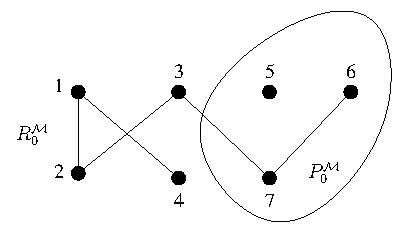
\includegraphics[width=0.4\linewidth]{figures/exercise-02-model.pdf}

    \smallskip
    \textsc{Kuva 1.} Malli
  \end{center}
\end{exercise}

\begin{solution}
  Disjunktion ja atomikaavojen totuusmääritelmien nojalla
  \[
    \begin{aligned}
      &\mathcal M \models_s \bigl(P_0(x) \lor R_0(y,z)\bigr) \\
      &\quad\text{joss}\quad
      \mathcal M \models_s P_0(x)
      \quad\text{tai}\quad
      \mathcal M \models_s R_0(y,z) \\
      &\quad\text{joss}\quad
      x^{\mathcal M}\langle s\rangle \in P_0^{\mathcal M}
      \quad\text{tai}\quad
      \bigl(y^{\mathcal M}\langle s\rangle,
      z^{\mathcal M}\langle s\rangle\bigr)
      \in R_0^{\mathcal M}.
    \end{aligned}
  \]
  Muuttujatermin arvo on \(x^{\mathcal M}\langle s\rangle = s(x)\),
  ja vastaavasti muuttujille \(y\) ja \(z\).

  Kuvasta nähdään, että \(P_0^{\mathcal M} = \{5,6,7\}\). Koska
  \[
    \begin{aligned}
      x^{\mathcal M}\langle s_0\rangle &= s_0(x) = 5
      \in P_0^{\mathcal M}, \\
      x^{\mathcal M}\langle s_1\rangle &= s_1(x) = 6
      \in P_0^{\mathcal M},
    \end{aligned}
  \]
  sekä \(s_0\) että \(s_1\) toteuttavat kaavan \(P_0(x)\) ja siten
  myös kaavan \(P_0(x) \lor R_0(y,z)\).

  Tulkintafunktiolle \(s_2\) sen sijaan pätee
  \[
    \begin{aligned}
      x^{\mathcal M}\langle s_2\rangle &= s_2(x) = 2
      \notin P_0^{\mathcal M}, \\
      \bigl(y^{\mathcal M}\langle s_2\rangle,
      z^{\mathcal M}\langle s_2\rangle\bigr)
      &= \bigl(s_2(y),s_2(z)\bigr) = (3,4)
      \notin R_0^{\mathcal M}.
    \end{aligned}
  \]
  Siis \(s_2\) ei toteuta kumpaakaan disjunktia, joten
  \(\mathcal M \not\models_{s_2} \bigl(P_0(x) \lor R_0(y,z)\bigr)\).
  Näin ollen annetuista tulkintafunktioista kaavan toteuttavat
  \textbf{täsmälleen \(s_0\) ja \(s_1\)}.
\end{solution}

\newpage

\begin{exercise}
  Olkoon \(L = \{P, R, c, d\}\), ja olkoon \(\mathcal M\) malli, jonka
  universumi on \(\NN\) ja jossa \(P^{\mathcal M} = 2\NN\) (eli parilliset
  luonnolliset luvut), \(R^{\mathcal M} = \{(0,1)\}\),
  \(c^{\mathcal M} = 1\) ja \(d^{\mathcal M} = 0\). Olkoon lisäksi \(s\)
  tulkintafunktio, jolla \(s(x_n) = n + 1\) kaikilla \(n \in \NN\).
  \begin{enumerate}[label=(\alph*)]
    \item Mikä on termin \(t\) arvo, kun
      \begin{enumerate}[label=(\alph*)]
        \item \(t = x_2\),
        \item \(t = c\),
        \item \(t = x_7\)?
      \end{enumerate}
    \item Toteuttaako tulkintafunktio \(s\) seuraavan kaavan mallissa
      \(\mathcal M\)?
      \begin{enumerate}[label=(\alph*)]
        \item \(P(x_8)\),
        \item \(P(x_1)\),
        \item \(R(c,d)\),
        \item \(R(d,x_0)\)?
      \end{enumerate}
  \end{enumerate}
\end{exercise}

\begin{solution}
  \leavevmode\par
  \begin{enumerate}[label=(\alph*)]
    \item Muuttujatermin arvon määrää tulkintafunktio \(s\), kun taas
      vakiosymbolin arvo on sen tulkinta mallissa \(\mathcal M\). Siten
      \[
        \begin{aligned}
          x_2^{\mathcal M}\langle s\rangle &= s(x_2) = 2 + 1 = 3, \\
          c^{\mathcal M}\langle s\rangle &= c^{\mathcal M} = 1, \\
          x_7^{\mathcal M}\langle s\rangle &= s(x_7) = 7 + 1 = 8.
        \end{aligned}
      \]

    \item Atomikaavojen totuusmääritelmän nojalla saadaan seuraavat
      vastaukset.
      \begin{enumerate}[label=(\alph*)]
        \item Kaava \(P(x_8)\) ei toteudu, sillä
          \[
            x_8^{\mathcal M}\langle s\rangle = s(x_8) = 9
            \notin P^{\mathcal M} = 2\NN.
          \]
          Siis \(\mathcal M \not\models_s P(x_8)\).

        \item Kaava \(P(x_1)\) toteutuu, sillä
          \[
            x_1^{\mathcal M}\langle s\rangle = s(x_1) = 2
            \in P^{\mathcal M} = 2\NN.
          \]
          Siis \(\mathcal M \models_s P(x_1)\).

        \item Kaava \(R(c,d)\) ei toteudu, sillä
          \[
            \bigl(c^{\mathcal M}\langle s\rangle,
            d^{\mathcal M}\langle s\rangle\bigr)
            = (1,0) \notin R^{\mathcal M} = \{(0,1)\}.
          \]
          Siis \(\mathcal M \not\models_s R(c,d)\).

        \item Kaava \(R(d,x_0)\) toteutuu, sillä
          \[
            \bigl(d^{\mathcal M}\langle s\rangle,
            x_0^{\mathcal M}\langle s\rangle\bigr)
            = (0,1) \in R^{\mathcal M} = \{(0,1)\}.
          \]
          Siis \(\mathcal M \models_s R(d,x_0)\).\qedhere
      \end{enumerate}
  \end{enumerate}
\end{solution}

\begin{exercise}
  Täytä tulkintafunktioiden arvot taulukkoon:
  \begin{center}
    \begin{tabular}{c|ccc}
      & \(x\) & \(y\) & \(z\) \\
      \hline
      \(s\) & 1 & 2 & 3 \\
      \(s(4/x)\) & 4 & 2 & 3 \\
      \(s(3/y)\) & 1 & 3 & 3 \\
      \(s(1/x)\) & 1 & 2 & 3 \\
      \(s(1/z)(1/y)\) & 1 & 1 & 1 \\
      \(s(3/x)(2/z)\) & 3 & 2 & 2 \\
      \(s(2/x)(3/y)(4/x)\) & 4 & 3 & 3
    \end{tabular}
  \end{center}
\end{exercise}

\begin{exercise}
  Mitkä seuraavista tulkintafunktioista toteuttavat kaavan
  \(E(x,y) \to E(y,z)\) kuvan 2 verkossa? Entä mitkä tulkintafunktioista
  toteuttavat kaavan \(E(x,y) \to \exists y\, E(y,z)\)? Anna perustelu.
  \begin{center}
    \begin{tabular}{c|ccc}
      & \(x\) & \(y\) & \(z\) \\
      \hline
      \(s_0\) & 1 & 2 & 3 \\
      \(s_1\) & 1 & 5 & 6 \\
      \(s_2\) & 4 & 8 & 8 \\
      \(s_3\) & 1 & 2 & 7 \\
      \(s_4\) & 1 & 2 & 5
    \end{tabular}

    \medskip
    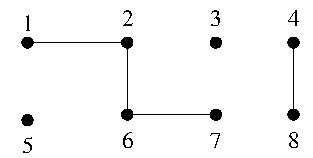
\includegraphics[width=0.3\linewidth]{figures/exercise-02-graph.pdf}

    \smallskip
    \textsc{Kuva 2.} Verkko
  \end{center}
\end{exercise}

\begin{solution}
  Implikaatio on epätosi vain, kun etujäsen on tosi ja takajäsen epätosi.
  Kaava \(\exists y\,E(y,z)\) toteutuu täsmälleen silloin, kun
  \(s(z)\notin\{3,5\}\), sillä vain solmut \(3\) ja \(5\) ovat
  eristettyjä. Sidotun muuttujan \(y\) alkuperäinen arvo ei vaikuta tähän.
  Taulukossa \(1\) tarkoittaa toteutumista ja \(0\) toteutumatta jäämistä.
  \begin{center}
    \renewcommand{\arraystretch}{1.15}
    \setlength{\tabcolsep}{4pt}
    \begin{tabular}{c|ccc|cc}
      & \(E(x,y)\) & \(E(y,z)\) & \(\exists y\,E(y,z)\)
      & \(E(x,y)\to E(y,z)\)
      & \(E(x,y)\to\exists y\,E(y,z)\) \\
      \hline
      \(s_0\) & 1 & 0 & 0 & 0 & 0 \\
      \(s_1\) & 0 & 0 & 1 & 1 & 1 \\
      \(s_2\) & 1 & 0 & 1 & 0 & 1 \\
      \(s_3\) & 1 & 0 & 1 & 0 & 1 \\
      \(s_4\) & 1 & 0 & 0 & 0 & 0
    \end{tabular}
  \end{center}
  Ensimmäisen kaavan toteuttaa siis vain \(s_1\), ja toisen kaavan
  täsmälleen \(s_1\), \(s_2\) ja \(s_3\).
\end{solution}

\begin{exercise}
  Anna \(\{E\}\)-kaava, joka verkossa ilmaisee (eli voit olettaa mallin olevan
  verkko), että jokaisella solmulla on ainakin kaksi eri naapuria. Kaksi verkon
  solmua ovat naapureita keskenään, jos niiden välissä on särmä.
\end{exercise}

\begin{solution}
  \[
    \forall x \exists y \exists z (\neg (y = z) \land E(x, y) \land E(x, z)).
  \]
\end{solution}

\begin{exercise}
  Ovatko seuraavat kaavat \textit{tosia} kuvan 2 verkossa? Perustele.
  \begin{enumerate}[label=(\alph*)]
    \item \(E(x,y)\)
    \item \(\exists x E(x,y)\)
    \item \(\exists x\exists y E(x,y)\)
    \item \(\exists y\exists z((E(x,y) \leftrightarrow E(x,z)) \land
      (E(x,y) \leftrightarrow E(y,z)))\)
  \end{enumerate}
\end{exercise}

\begin{solution}
  Merkitään kuvan 2 verkkoa mallilla \(\mathcal M\). Kaava \(A\) on
  tosi mallissa \(\mathcal M\), eli \(\mathcal M\models A\), jos
  \(\mathcal M\models_s A\) kaikilla \(\mathcal M\)-tulkintafunktioilla
  \(s\). Siksi yksi vastaesimerkki riittää osoittamaan, ettei kaava ole
  tosi mallissa.
  \leavevmode\par
  \begin{enumerate}[label=(\alph*)]
    \item Kaava \(E(x,y)\) \textbf{ei ole tosi}. Valitaan
      tulkintafunktio \(s\), jolla \(s(x)=1\) ja \(s(y)=5\).
      Solmujen \(1\) ja \(5\) välillä ei ole särmää, joten
      \[
        (s(x),s(y))=(1,5)\notin E^{\mathcal M}.
      \]
      Siis \(\mathcal M\not\models_s E(x,y)\), joten
      \(\mathcal M\not\models E(x,y)\).

    \item Kaava \(\exists x\,E(x,y)\) \textbf{ei ole tosi}.
      Valitaan tulkintafunktio \(s\), jolla \(s(y)=3\).
      Koska solmu \(3\) on eristetty, kaikilla
      \(a\in\dom(\mathcal M)\) pätee
      \[
        \bigl(x^{\mathcal M}\langle s(a/x)\rangle,
        y^{\mathcal M}\langle s(a/x)\rangle\bigr)
        =(a,3)\notin E^{\mathcal M}.
      \]
      Näin ollen \(\mathcal M\not\models_{s(a/x)} E(x,y)\)
      kaikilla \(a\in\dom(\mathcal M)\). Eksistenssikvanttorin
      totuusmääritelmän nojalla
      \(\mathcal M\not\models_s\exists x\,E(x,y)\), joten
      \(\mathcal M\not\models\exists x\,E(x,y)\).

    \item Kaava \(\exists x\exists y\,E(x,y)\) \textbf{on tosi}.
      Olkoon \(s\) mielivaltainen \(\mathcal M\)-tulkintafunktio.
      Valitaan eksistenssikvanttorien todistajiksi \(a=1\) ja \(b=2\).
      Tulkintafunktiolle \(s'=s(1/x)(2/y)\) pätee
      \[
        (s'(x),s'(y))=(1,2)\in E^{\mathcal M},
      \]
      sillä solmujen \(1\) ja \(2\) välillä on särmä. Siis
      \(\mathcal M\models_{s'}E(x,y)\), joten
      \(\mathcal M\models_s\exists x\exists y\,E(x,y)\).
      Koska \(s\) oli mielivaltainen,
      \[
        \mathcal M\models\exists x\exists y\,E(x,y).
      \]

    \item Kaava \textbf{on tosi}. Olkoon \(s\) mielivaltainen
      \(\mathcal M\)-tulkintafunktio. Valitaan molempien
      eksistenssikvanttorien todistajaksi solmu \(3\), eli asetetaan
      \(s'=s(3/y)(3/z)\). Koska solmu \(3\) on eristetty,
      \[
        \begin{aligned}
          (s'(x),s'(y))&=(s(x),3)\notin E^{\mathcal M},\\
          (s'(x),s'(z))&=(s(x),3)\notin E^{\mathcal M},\\
          (s'(y),s'(z))&=(3,3)\notin E^{\mathcal M}.
        \end{aligned}
      \]
      Kaavat \(E(x,y)\), \(E(x,z)\) ja \(E(y,z)\) ovat siis
      kaikki epätosia tulkinnalla \(s'\). Ekvivalenssi on tosi,
      kun sen molemmilla puolilla on sama totuusarvo, joten
      \[
        \mathcal M\models_{s'}
        \bigl((E(x,y)\leftrightarrow E(x,z))\land
        (E(x,y)\leftrightarrow E(y,z))\bigr).
      \]
      Eksistenssikvanttorien totuusmääritelmän ja tulkintafunktion
      \(s\) mielivaltaisuuden nojalla
      \[
        \mathcal M\models\exists y\exists z
        \bigl((E(x,y)\leftrightarrow E(x,z))\land
        (E(x,y)\leftrightarrow E(y,z))\bigr).
      \]
      Valinta \(y=z=3\) on sallittu, sillä kaava ei edellytä
      todistajien olevan eri solmuja.\qedhere
  \end{enumerate}
\end{solution}

\begin{samepage}
  \begin{exercise}
    Anna esimerkki kaavasta \(A\) tai selitä, miksi sellaista ei ole,
    kun \(A\) on
    \begin{enumerate}[label=(\alph*)]
      \item toteutuva muttei validi,
      \item kumoutuva muttei ristiriita,
      \item tautologia muttei validi,
      \item validi muttei tautologia.
    \end{enumerate}
  \end{exercise}
\end{samepage}

\begin{solution}
  \leavevmode\par
  \begin{enumerate}[label=(\alph*)]
    \item Valitaan \(A=(x=y)\). Olkoon \(\mathcal M\) malli, jonka
      universumi on \(\{1\}\), ja olkoon \(s\) sen tulkintafunktio.
      Tällöin \(s(x)=s(y)=1\), joten
      \[
        \mathcal M\models_s x=y.
      \]
      Kaava on siis toteutuva. Se ei kuitenkaan ole validi:
      valitaan malli \(\mathcal N\), jonka universumi on \(\{1,2\}\),
      ja tulkintafunktio \(t\), jolla \(t(x)=1\) ja \(t(y)=2\).
      Koska \(t(x)\ne t(y)\), saadaan
      \[
        \mathcal N\not\models_t x=y.
      \]

    \item Myös tässä \(A=(x=y)\) toimii. Kohdan (a) malli
      \(\mathcal N\) ja tulkintafunktio \(t\) osoittavat, että kaava
      on kumoutuva, sillä \(\mathcal N\not\models_t A\).
      Toisaalta \(\mathcal M\models_s A\), joten kaava on toteutuva
      eikä siten ristiriita.

    \item Tällaista kaavaa ei ole, sillä jokainen tautologia on
      validi. Tautologian totuus seuraa sen propositionaalisesta
      muodosta riippumatta osakaavojen totuusarvoista. Siksi se
      toteutuu jokaisessa mallissa jokaisella tulkintafunktiolla.

    \item Valitaan \(A=\forall x\,(x=x)\). Olkoon \(\mathcal M\)
      mielivaltainen malli ja \(s\) sen mielivaltainen
      tulkintafunktio. Kaikilla \(a\in\dom(\mathcal M)\) pätee
      \[
        x^{\mathcal M}\langle s(a/x)\rangle
        =a
        =x^{\mathcal M}\langle s(a/x)\rangle,
      \]
      joten \(\mathcal M\models_{s(a/x)}x=x\).
      Universaalikvanttorin totuusmääritelmän nojalla
      \(\mathcal M\models_s\forall x\,(x=x)\).
      Koska \(\mathcal M\) ja \(s\) olivat mielivaltaisia,
      kaava on validi.

      Kaava ei kuitenkaan ole tautologia. Sen propositionaalinen
      muoto on pelkkä propositiosymboli \(p\), joka ei ole
      propositiologiikan tautologia: se on epätosi arvotuksella,
      jossa \(p\) saa totuusarvon \(0\). Kaavan \(A\) validius
      perustuu yhtäsuuruuden ja kvanttorin semantiikkaan.\qedhere
  \end{enumerate}
\end{solution}

\begin{exercise}
  \leavevmode
  \begin{enumerate}[label=(\alph*)]
    \item Osoita, että kaava \(\exists x P(x)\) on kaavan \(\forall x P(x)\)
      looginen seuraus.
    \item Osoita, että kaavat \(\exists x P(x)\) ja \(\forall x P(x)\) eivät ole
      loogisesti ekvivalentit.
  \end{enumerate}
\end{exercise}

\begin{solution}
  \leavevmode\par
  \begin{enumerate}[label=(\alph*)]
    \item Olkoon \(\mathcal M\) mielivaltainen \(\{P\}\)-malli ja
      \(s\) sen mielivaltainen tulkintafunktio. Oletetaan, että
      \(\mathcal M\models_s\forall x\,P(x)\).
      Universaalikvanttorin totuusmääritelmän nojalla
      \[
        \mathcal M\models_{s(a/x)}P(x)
        \quad\text{kaikilla }a\in\dom(\mathcal M).
      \]
      Mallin universumi on epätyhjä, joten voidaan valita
      \(a_0\in\dom(\mathcal M)\). Erityisesti
      \(\mathcal M\models_{s(a_0/x)}P(x)\), joten
      eksistenssikvanttorin totuusmääritelmän nojalla
      \[
        \mathcal M\models_s\exists x\,P(x).
      \]
      Koska \(\mathcal M\) ja \(s\) olivat mielivaltaisia, on osoitettu,
      että
      \[
        \forall x\,P(x)\models\exists x\,P(x).
      \]

    \item Valitaan \(\{P\}\)-malli \(\mathcal M\), jossa
      \[
        \dom(\mathcal M)=\NN,
        \qquad
        P^{\mathcal M}=\{n\in\NN\mid n\text{ on alkuluku}\}.
      \]
      Olkoon \(s\) mielivaltainen \(\mathcal M\)-tulkintafunktio.
      Koska \(2\) on alkuluku, saadaan
      \[
        x^{\mathcal M}\langle s(2/x)\rangle
        =2\in P^{\mathcal M}.
      \]
      Siis \(\mathcal M\models_{s(2/x)}P(x)\), joten
      \(\mathcal M\models_s\exists x\,P(x)\).
      Toisaalta \(4\) ei ole alkuluku, joten
      \[
        x^{\mathcal M}\langle s(4/x)\rangle
        =4\notin P^{\mathcal M}.
      \]
      Näin ollen \(\mathcal M\not\models_{s(4/x)}P(x)\), joten
      \(\mathcal M\not\models_s\forall x\,P(x)\).
      Kaavoilla on siis eri totuusarvot samassa mallissa samalla
      tulkintafunktiolla. Siksi ne eivät ole loogisesti
      ekvivalentit.\qedhere
  \end{enumerate}
\end{solution}

\end{document}
